\documentclass{beamer}
\usepackage{graphicx}
\usepackage{amsmath, amsthm, amsfonts, amssymb, mathrsfs}
\usepackage{textcomp} % straigth apos
\usepackage{tikz}
\usepackage{verbatim}
\usepackage{tikzit}
\usepackage{listings}
\usepackage{subfig}
\usepackage[ruled,vlined, linesnumbered]{algorithm2e}
\usepackage{algorithmic,float}


\input{graphs.tikzstyles}

% Graph notations
\def\NN{$\mathcal{N}~$}
\def\GG{$\mathcal{G}~$}
\def\VV{$\mathcal{V}~$}
\def\EE{$\mathcal{E}~$}


% Colors definition
\definecolor{isa_red}{RGB}{255, 58, 71}
\definecolor{isa_blue}{RGB}{0, 103, 158}
\definecolor{isa_green}{RGB}{0, 157, 97}
\definecolor{isa_dark_green}{RGB}{0,131, 0}
\definecolor{isa_purple}{RGB}{174, 5, 238}
\definecolor{isa_dark_blue}{RGB}{26, 0, 253}

% Isabelle keywords
\newcommand{\apply}{{\color{isa_red}{apply}}}
\newcommand{\done}{{\color{isa_red}{done}}}
\newcommand{\datatype}{{\color{isa_blue}{datatype}}}
\newcommand{\inductive}{{\color{isa_blue}{inductive}}}
\newcommand{\abbreviation}{{\color{isa_blue}{abbreviation}}}
\newcommand{\thm}{{\color{isa_blue}{theorem}}}
\newcommand{\lm}{{\color{isa_blue}{lemma}}}
\newcommand{\fun}{{\color{isa_blue}{fun}}}
\renewcommand{\locale}{{\color{isa_blue}{locale}}}
\newcommand{\where}{{\color{isa_green}{where}}}
\renewcommand{\and}{{\color{isa_green}{and}}}
\newcommand{\fixes}{{\color{isa_green}{fixes}}}
\newcommand{\assumes}{{\color{isa_green}{assumes}}}
\newcommand{\shows}{{\color{isa_green}{shows}}}
\newcommand{\generic}[1]{{\color{isa_purple}{\textquotesingle#1}}}
\newcommand{\isa}[1]{\texttt{#1}}
\newcommand{\blue}[1]{{\color{isa_dark_blue}{#1}}}
\newcommand{\green}[1]{{\color{isa_dark_green}{#1}}}

\theoremstyle{definition}
\newtheorem*{isabelle}{}

\setbeamercovered{invisible}

\setbeamertemplate{theorems}[numbered]
\setbeamertemplate{lemma}[numbered]
\newtheorem{remark}{Remark}

\usetheme{Madrid}
\useoutertheme{tree} % Alternatively: miniframes, infolines, split
\useinnertheme{circles}

\setbeamertemplate{headline}
{%
  \leavevmode%
  \begin{beamercolorbox}[wd=.5\paperwidth,ht=2.5ex,dp=1.125ex]{section in head/foot}%
    \hbox to .5\paperwidth{\hfil\insertsectionhead\hfil}
  \end{beamercolorbox}%
  \begin{beamercolorbox}[wd=.5\paperwidth,ht=2.5ex,dp=1.125ex]{subsection in head/foot}%
    \hbox to .5\paperwidth{\hfil\insertsubsectionhead\hfil}
  \end{beamercolorbox}%
}

\definecolor{lightbrown}{RGB}{220, 147, 91}

\usecolortheme[named=lightbrown]{structure}

\title[Vérification formelle en Isabelle]{Vérification formelle en Isabelle(HOL)\\d'un algorithme calculant les composantes\\ fortement connexes d'un graphe}
%% sm: not really convinced by the title -- FM in HOL sounds redundant to me
%% also are there really several algorithms?
%% maybe "Verification in HOL of an algorithm for computing SCCs" ?
\date{June 9, 2022}
\author[V. Trélat, S. Merz]{Vincent Trélat\\encadré par Stephan Merz}
\institute[Mines Nancy]{\normalsize{École Nationale Supérieure des Mines de Nancy\\Département Informatique}}

\begin{document}

\begin{frame}
  \begin{figure}[t]
    \centering
    
\includegraphics[height=30pt]{img/logoartem.png}
    \hspace{1cm}
    
\includegraphics[height=32pt]{img/logoloria.jpg}
    \hspace{1cm}
    
\includegraphics[height=32pt]{img/logoisabelle.png}
  \end{figure}
  \titlepage
\end{frame}

\section{Présentation et intérêt des méthodes formelles}
\begin{frame}
  \tableofcontents
\end{frame}

\subsection{Programmation défensive}
\begin{frame}
    \onslide<1->{
        \begin{center}
            Comment garantir le fonctionnement continu d'un logiciel dans des conditions imprévues ?
        \end{center}
        \vfill
    }
    \begin{itemize}
        \item<2-> Concepts de Software Engineering (design documents, design patterns, etc.)
        \item<2-> Review de code en équipe (GitHub, etc.)
        \item<2-> Séries de tests (unitaires, d'intégration, fonctionnels, etc.)
    \end{itemize}
    \vfill
    \onslide<3->{
        $\Longrightarrow$ Responsabilité du programmeur !
    }
\end{frame}

\begin{frame}
    \onslide<1->{
        \begin{quotation}
            Probability of human error is considerably higher than that of machine error.
            \begin{flushright}
                Kenneth Appel
        \end{flushright}
        % Kenneth Appel est un mathématicien qui a démontré le théorème des 4 couleurs (problème 4-COL) en 1976 :
        % Il est possible, en n'utilisant que 4 couleurs, de colorier n'importe quelle carte découpée en régions connexes, de sortes que deux régions adjacentes soient toujours de couleur différente.
    \end{quotation}
    }
    \onslide<2->{
        \begin{figure}
            \centering
            \subfloat{
                
\includegraphics[height=3.5cm]{img/4col.png}
            }
            \subfloat{
                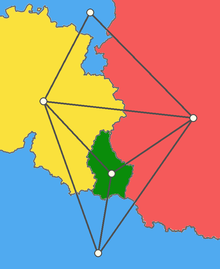
\includegraphics[height=3.5cm]{img/4col2.png}
            }
        \caption{Illustrations du problème 4-COL}
        \end{figure}
    % Première preuve assistée par ordinateur ! Explosion combinatoire dûe au nombre de cas à explorer. Débat à l'époque sur la validité de la preuve.
    }
\end{frame}

\subsection{Les méthodes formelles}
\begin{frame}
    En méthodes formelles, on considère un programme comme une structure mathématique, ce qui permet de raisonner dessus de manière formelle.
    % les méthodes formelles sont des techniques permettant de raisonner rigoureusement, à l'aide de logique mathématique, sur un programme informatique, afin de démontrer sa validité par rapport à une certaine spécification. Elles reposent sur la sémantique des programmes, c'est-à-dire sur des descriptions mathématiques formelles du sens d'un programme donné par son code.
    \vfill
    \begin{itemize}
        \item Rigueur
        \item Concepts de logique
        \item Validité par rapport à des spécifications
        \item Sémantique
    \end{itemize}
\end{frame}

\begin{frame}
    \begin{center}
        Preuve papier vs. preuve formelle
    \end{center}
    \begin{itemize}
        \item L'utilisateur fournit la structure de la preuve
        \item Automatisation des preuves
        \item Différents outils informatiques : assistants à la preuve (Isabelle(HOL), Coq, Why3, B, etc.) et model checkers (TLC, etc.)
    \end{itemize}
\end{frame}

\subsection{Applications}
\begin{frame}
    \frametitle{Quelles applications ?}
    Éviter les ``bugs'' : applications aux systèmes critiques
    \vfill
    Ex: Ariane 5, Entreprise Clearsy
    \begin{figure}
        \subfloat{
        \begin{minipage}{0.35\textwidth}
            \centering
            
\includegraphics[width=.9\textwidth]{img/logoclearsy.png}
        \end{minipage}
        }
        \subfloat{
            \begin{minipage}{0.6\textwidth}
                Application au milieu ferroviaire :
                Certification du logiciel de pilotage automatique des lignes 1 et 14 de métro à Paris, bientôt la ligne 4
            \end{minipage}
        }
    \end{figure}
\end{frame}

\section{Introduction du projet}
\subsection{Définition}
\begin{frame}
    \tableofcontents[currentsection]
  \end{frame}

\begin{frame}
    \frametitle{Composante fortement connexe}
    \onslide<1->{
        \begin{definition}[SCC]
            Soient $\mathcal{G} := (\mathcal{V}, \mathcal{E})$ un \blue{graphe orienté} et $\mathcal{C} \subseteq \mathcal{V}$.
            $\mathcal{C}$ est une SCC de $\mathcal{G}$ si:
            \begin{equation*}
            \forall x, y \in \mathcal{C}, (x \Rightarrow^* y) \wedge (y \Rightarrow^* x)
            \end{equation*}
            % Définition redondante mais plus facile à comprendre.
        \end{definition}
    }
    \only<1-2>{
        \uncover<2>{
        \ctikzfig{slides_sccex1}
        }
    }
    \only<3>{
        \ctikzfig{slides_sccex3}
    }
    \only<4>{
        \ctikzfig{slides_sccex2}
    }
    \only<5>{
        \ctikzfig{slides_sccex4}
    }
\end{frame}

\subsection{Motivation du problème}
\begin{frame}
    \ctikzfig{biggraph}
    \onslide<1->{
      \begin{itemize}
        \item Réseaux: interconnectivité et partage de données
        \item Model checking: recherche de contre-exemples
      \end{itemize}
    }
    \vfill
    \onslide<2->{
      Algorithmes efficaces (ex: Tarjan)
      \begin{itemize}
        \item La vérification formelle de leur correction est utile
        \item Un autre défi : la parallélisation
        % Lien avec la preuve actuelle
      \end{itemize}
    }
    \end{frame}

\section{Vérification formelle en Isabelle}
\subsection{Présentation de l'algorithme}
\begin{frame}
    \tableofcontents[currentsection]
\end{frame}

\setbeamercovered{transparent}
\begin{frame}[fragile]
\onslide<1->{
\fboxsep=0pt
\noindent{%
\begin{minipage}[c]{0.48\linewidth}
  \setlength{\interspacetitleruled}{0pt}%
  \setlength{\algotitleheightrule}{0pt}%
  \begin{algorithm}[H]
    \tiny
    \uncover<1, 12>{
    \KwData{A graph \GG = (\VV, \EE), a starting node $v_0$\;}
    Initialize an empty set \texttt{VISITED}\;
    Initialize an empty set \texttt{EXPLORED}\;
    Initialize an empty stack \texttt{R}\;
    setBased($v_0$)\;
    }
    \SetKwProg{Function}{function}{}{}
    \uncover<2->{
    \Function{setBased: $v \in \mathcal{V} \rightarrow \texttt{None}$}{
      $\texttt{VISITED} := \texttt{VISITED} \cup \{v\}$\;
      \texttt{R.push($v$)}\;
        \ForEach{$w\in \texttt{POST(v)}$}{
            \If{$w\in \texttt{EXPLORED}$}{
                continue\;
            }
            \ElseIf{$w \notin \texttt{VISITED}$}{
                setBased($w$)\;
            }
            \Else{
                \While{$\mathcal{S}(v) \neq \mathcal{S}(w)$}{
                    $r := \texttt{R.pop()}$\;
                    $\texttt{UNITE}(\mathcal{S}, r, \texttt{R.top()})$\;
                }
            }
        }
        \If{$v = \texttt{R.top()}$}{
            \textbf{report SCC} $\mathcal{S}(v)$\;
            $\texttt{EXPLORED} := \texttt{EXPLORED} \cup \mathcal{S}(v)$\;
            \texttt{R.pop()}\;
        }
    }
    }
  \end{algorithm}
\end{minipage}}%
}
\hfill%
{%
\begin{minipage}[c]{0.48\linewidth}
\only<+>{
  \ctikzfig{slides_seqalg1}
}
\only<+>{
  \ctikzfig{slides_seqalg2}
}
\only<+>{
  \ctikzfig{slides_seqalg3}
}
\only<+>{
  \ctikzfig{slides_seqalg4}
}
\only<+>{
  \ctikzfig{slides_seqalg5}
}
\only<+>{
  \ctikzfig{slides_seqalg6}
}
\only<+>{
  \ctikzfig{slides_seqalg7}
}
\only<+>{
  \ctikzfig{slides_seqalg8}
}
\only<+>{
  \ctikzfig{slides_seqalg9}
}
\only<+>{
  \ctikzfig{slides_seqalg10}
}
\only<+>{
  \ctikzfig{slides_seqalg11}
}
\only<+>{
  \ctikzfig{slides_seqalg12}
}
\end{minipage}
}
\end{frame}

\subsection{Structure de la preuve}
\begin{frame}
    \tableofcontents[currentsection, currentsubsection]
\end{frame}

\begin{frame}
    \begin{itemize}
        \item Modélisation et implémentation de l'algorithme
        \begin{itemize}
            \item[$\circ$] Définition de l'environnement
            \item[$\circ$] Fonctions \texttt{unite}, \texttt{dfs} et \texttt{dfss}
        \end{itemize}
        \vfill
        \item Définition des invariants
        \begin{itemize}
          \item[$\circ$] définitions : \texttt{reachable} et \texttt{is\_scc}
          \item[$\circ$] well-formed environment
          \item[$\circ$] pré-conditions et post-conditions sur \texttt{dfs} et \texttt{dfss}
        \end{itemize}
        \vfill
        \item Écriture et preuve des lemmes
        \begin{itemize}
            \item[$\circ$] $\texttt{pre\_dfs} \Longrightarrow \texttt{pre\_dfss}$
            \item[$\circ$] $\texttt{pre\_dfss} \Longrightarrow \texttt{pre\_dfs}$
            \item[$\circ$] $\texttt{pre\_dfs} \Longrightarrow \texttt{post\_dfs}$
            \item[$\circ$] $\texttt{pre\_dfss} \Longrightarrow \texttt{post\_dfss}$
            \item[$\circ$] théorème final
            % bien insister sur la dépendance mutuelle des différents lemmes car les fonctions sont mutuellement récursives
        \end{itemize}
    \end{itemize}    
\end{frame}

\section{Conclusion}
\begin{frame}
    \tableofcontents[currentsection]
\end{frame}

\begin{frame}
    \begin{itemize}
        \item Ce qui a été fait :
        \begin{itemize}
          \item[$\circ$] Modèle cohérent et stable
          \item[$\circ$] Preuve de tous les lemmes intermédiaires (ou presque)
        \end{itemize}
        \vfill
        \item Ce qui manque :
        \begin{itemize}
          \item[$\circ$] Quelques propriétés intermédiaires sont à démontrer
          \item[$\circ$] Théorème final
          \item[$\circ$] Montrer la terminaison
        \end{itemize}
    \end{itemize}
\end{frame}

\end{document}